\documentclass[journal,12pt,twocolumn]{IEEEtran}

\usepackage{setspace}
\usepackage{gensymb}

\singlespacing


\usepackage[cmex10]{amsmath}

\usepackage{amsthm}

\usepackage{mathrsfs}
\usepackage{txfonts}
\usepackage{stfloats}
\usepackage{bm}
\usepackage{cite}
\usepackage{cases}
\usepackage{subfig}

\usepackage{longtable}
\usepackage{multirow}

\usepackage{enumitem}
\usepackage{mathtools}
\usepackage{steinmetz}
\usepackage{tikz}
\usepackage{circuitikz}
\usepackage{verbatim}
\usepackage{tfrupee}
\usepackage[breaklinks=true]{hyperref}
\usepackage{graphicx}
\usepackage{tkz-euclide}
\usepackage{float}

\usetikzlibrary{calc,math}
\usepackage{listings}
    \usepackage{color}                                            %%
    \usepackage{array}                                            %%
    \usepackage{longtable}                                        %%
    \usepackage{calc}                                             %%
    \usepackage{multirow}                                         %%
    \usepackage{hhline}                                           %%
    \usepackage{ifthen}                                           %%
    \usepackage{lscape}     
\usepackage{multicol}
\usepackage{chngcntr}

\DeclareMathOperator*{\Res}{Res}

\renewcommand\thesection{\arabic{section}}
\renewcommand\thesubsection{\thesection.\arabic{subsection}}
\renewcommand\thesubsubsection{\thesubsection.\arabic{subsubsection}}

\renewcommand\thesectiondis{\arabic{section}}
\renewcommand\thesubsectiondis{\thesectiondis.\arabic{subsection}}
\renewcommand\thesubsubsectiondis{\thesubsectiondis.\arabic{subsubsection}}


\hyphenation{op-tical net-works semi-conduc-tor}
\def\inputGnumericTable{}                                 %%

\lstset{
%language=C,
frame=single, 
breaklines=true,
columns=fullflexible
}
\begin{document}
\newtheorem{theorem}{Theorem}[section]
\newtheorem{problem}{Problem}
\newtheorem{proposition}{Proposition}[section]
\newtheorem{lemma}{Lemma}[section]
\newtheorem{corollary}[theorem]{Corollary}
\newtheorem{example}{Example}[section]
\newtheorem{definition}[problem]{Definition}

\newcommand{\BEQA}{\begin{eqnarray}}
\newcommand{\EEQA}{\end{eqnarray}}
\newcommand{\define}{\stackrel{\triangle}{=}}
\bibliographystyle{IEEEtran}
\providecommand{\mbf}{\mathbf}
\providecommand{\pr}[1]{\ensuremath{\Pr\left(#1\right)}}
\providecommand{\qfunc}[1]{\ensuremath{Q\left(#1\right)}}
\providecommand{\sbrak}[1]{\ensuremath{{}\left[#1\right]}}
\providecommand{\lsbrak}[1]{\ensuremath{{}\left[#1\right.}}
\providecommand{\rsbrak}[1]{\ensuremath{{}\left.#1\right]}}
\providecommand{\brak}[1]{\ensuremath{\left(#1\right)}}
\providecommand{\lbrak}[1]{\ensuremath{\left(#1\right.}}
\providecommand{\rbrak}[1]{\ensuremath{\left.#1\right)}}
\providecommand{\cbrak}[1]{\ensuremath{\left\{#1\right\}}}
\providecommand{\lcbrak}[1]{\ensuremath{\left\{#1\right.}}
\providecommand{\rcbrak}[1]{\ensuremath{\left.#1\right\}}}
\theoremstyle{remark}
\newtheorem{rem}{Remark}
\newcommand{\sgn}{\mathop{\mathrm{sgn}}}
\providecommand{\abs}[1]{\vert#1\vert}
\providecommand{\res}[1]{\Res\displaylimits_{#1}} 
\providecommand{\norm}[1]{\lVert#1\rVert}
%\providecommand{\norm}[1]{\lVert#1\rVert}
\providecommand{\mtx}[1]{\mathbf{#1}}
\providecommand{\mean}[1]{E[ #1 ]}
\providecommand{\fourier}{\overset{\mathcal{F}}{ \rightleftharpoons}}
%\providecommand{\hilbert}{\overset{\mathcal{H}}{ \rightleftharpoons}}
\providecommand{\system}{\overset{\mathcal{H}}{ \longleftrightarrow}}
	%\newcommand{\solution}[2]{\textbf{Solution:}{#1}}
\newcommand{\solution}{\noindent \textbf{Solution: }}
\newcommand{\cosec}{\,\text{cosec}\,}
\providecommand{\dec}[2]{\ensuremath{\overset{#1}{\underset{#2}{\gtrless}}}}
\newcommand{\myvec}[1]{\ensuremath{\begin{pmatrix}#1\end{pmatrix}}}
\newcommand{\mydet}[1]{\ensuremath{\begin{vmatrix}#1\end{vmatrix}}}
\numberwithin{equation}{subsection}
\makeatletter
\@addtoreset{figure}{problem}
\makeatother
\let\StandardTheFigure\thefigure
\let\vec\mathbf
\renewcommand{\thefigure}{\theproblem}
\def\putbox#1#2#3{\makebox[0in][l]{\makebox[#1][l]{}\raisebox{\baselineskip}[0in][0in]{\raisebox{#2}[0in][0in]{#3}}}}
     \def\rightbox#1{\makebox[0in][r]{#1}}
     \def\centbox#1{\makebox[0in]{#1}}
     \def\topbox#1{\raisebox{-\baselineskip}[0in][0in]{#1}}
     \def\midbox#1{\raisebox{-0.5\baselineskip}[0in][0in]{#1}}
\vspace{3cm}
\title{ASSIGNMENT 3}
\author{Dishank Jain \\ AI20BTECH11011}
\maketitle
\newpage
\bigskip
\renewcommand{\thefigure}{\theenumi}
\renewcommand{\thetable}{\theenumi}
Download all python codes from 
\begin{lstlisting}
https://github.com/Dishank422/EE3900/blob/main/assignment3/codes
\end{lstlisting}
%
and latex-tikz codes from 
%
\begin{lstlisting}
https://github.com/Dishank422/EE3900/blob/main/assignment3/Assignment3.tex
\end{lstlisting}
%
\section{Constructions Q2.4}
Construct a quadrilateral ABCD such that BC = 4.5, AC = 5.5, CD = 5, BD = 7  and AD = 5.5.
\section{Solution}
Using AC = 5.5,
\begin{align}
    Let\; \vec{A} &= \myvec{0\\0},\; \vec{C} = \myvec{5.5\\0}\\
    \vec{B} &= \myvec{x\\y},\; \vec{D} = \myvec{h\\k}
\end{align}

We know 
\begin{align}
    \norm{\vec{D}-\vec{A}} &= 5.5\label{DA}\\
    \norm{\vec{D}-\vec{C}} &= 5\label{DC}\\
    \norm{\vec{B}-\vec{C}} &= 4.5\label{BC}\\
    \norm{\vec{B}-\vec{D}} &= 7\label{BD}
\end{align}
\begin{align}
    h &= \dfrac{AC^2+AD^2-CD^2}{2AC}\\
      &= \dfrac{5.5^2+5.5^2-5^2}{2\times 5.5}\\
      &= 3.23\\
    k &= \sqrt{(AD^2-h^2)}\\
      &= \sqrt{(5.5^2-h^2)}\\
      &= 4.45\\
    \implies \vec{D} &= \myvec{3.23\\4.45}
\end{align}
Note: Above computations can be found in codes/finding\textunderscore D.py.

From \ref{BC} and \ref{BD},
\begin{align}
    &(x-5.5)^2+(y-0)^2 =4.5^2\\
    (&x-3.23)^2+(y-4.45)^2 =7^2\\
    \implies &x^2-11x+30.25+y^2=20.25\\
    \implies &x^2-6.46x+10.43+y^2-8.9y+19.8=49\\
    \implies &4.34x-8.9y=28.77\\
    \implies &y = 0.49x-3.23\\
    \implies &x^2-11x+30.25+(0.49x-3.23)^2 = 20.25\\
    \implies &1.24x^2-14.17x+0.43=0\\
    \implies &x = 0.03, 11.4\\
    \implies &y = -3.22, 2.37
\end{align}

Note: The values of x are found using codes/quadratic\textunderscore solve.py. Since $\vec{A}$, $\vec{B}$, $\vec{C}$ and $\vec{D}$ are in that order, 
\begin{equation}
    \vec{B} = \myvec{0.03\\-3.22}
\end{equation}

Using the co-ordinates of the vertices as found, the following quadrilateral is plotted.
\begin{figure}[h]
    \resizebox{\columnwidth}{!}{
    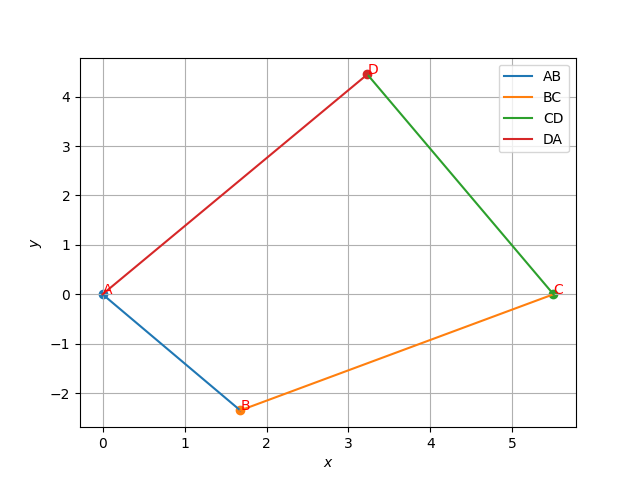
\includegraphics{figures/figure.png}
    }
    %\caption{Required quadrilateral}
    %\label{quad_plot}
\end{figure}
\end{document}
